

\section{Introduktion} %%%%%%%%%%%%%%%%%%%%%%%%%%%%%%%%%%%%%%%%%%%%%%%%%%%%%%%%%%%%
%%%%%%%%%%%% MID WAY AGENDA %%%%%%%%%%%%%%
%\begin{frame}<beamer>
%\frametitle{Simon Bjerre Krogh}
%\tableofcontents[currentsection]
%\end{frame}


% the license
\subsection{Kloakker og rensningsanlæg generelt} %%%%%%%%%%%%%%%%%%%%%%%%
\begin{frame}{Typisk opbygning af kloak ledning}{}
\vfill\vfill\centering
\begin{figure}[H]
\centering
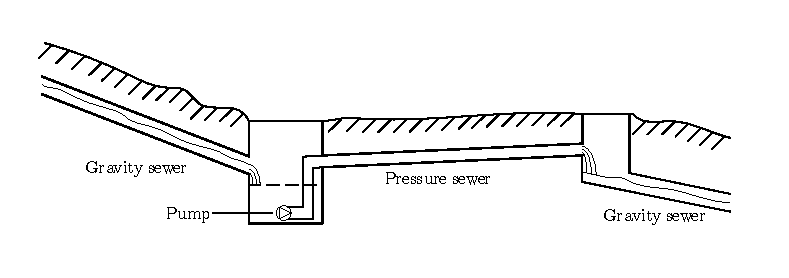
\includegraphics[width=1\textwidth]{Sections/pictures/Sewer_drawing.pdf}
\end{figure}
\vfill\vfill
\end{frame}
%
%\subsection{Rensningsanlæg} %%%%%%%%%%%%%%%%%%%%%%%%%%

\begin{frame}{Tilstande i kloakken}
\vfill\vfill\centering
\begin{itemize}
	\item<1-> Aerob $\rightarrow$ $O_2$ $\rightarrow$ $H_2O$
	\item<2-> Anaerob $\rightarrow$ $SO_4^{-2}$ $\rightarrow$ $H_2S$
	\item<3-> Anoxisk $\rightarrow$ $NO_3^-$ $\rightarrow$ $N_2$
\end{itemize}
\vfill\vfill	
\end{frame}

\begin{frame}{Udfordringer ved spildevands rensning}{}
\vfill\vfill\centering
\begin{itemize}
	\item Virksomheds besøg ved Fredericia Spildevand og Energi A/S.
	
	\begin{itemize}
		\item<1-> Større udledninger uden varsel
		\item<2-> Problemer for aerobe bakterier
		\item<3-> Andre forstyrelser
	\end{itemize}	

\end{itemize}
\vfill\vfill
\end{frame}

\subsection{Problem formulering}

\begin{frame}{Problem formulering}{}
\vfill\vfill\centering
How can a simulation environment be constructed, which mimic the behavior of a real
sewer system, where MPC is utilized as the control scheme to obtain stable sewage output
such that optimal performance can be obtained from a WWTP.
\vfill\vfill
\end{frame}

\section{System beskrivelse} %%%%%%%%%%%%%%%%%%%%%%%%%%%%%%%%%%%%%%%%%%%%%%%%%%%%%%%%%%%%%%%%%%

%\subsection{Udgangspunkt i et virkeligt setup} %%%%%%%

\begin{frame}{Udgangspunkt i et virkeligt setup}{}
%\centering
\begin{figure}[H]
\centering
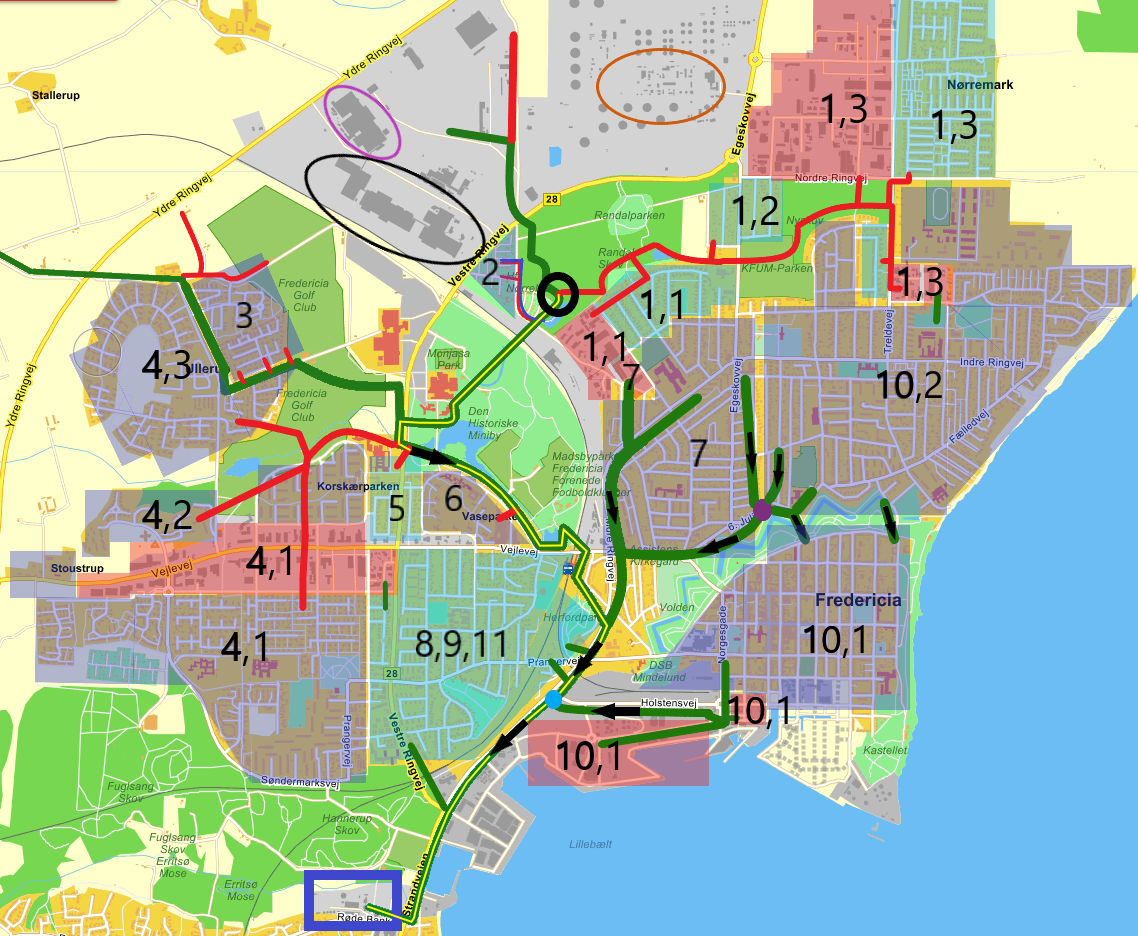
\includegraphics[width=0.7\textwidth]{Sections/pictures/kloakgrid_simplified10.png}
\end{figure}
%\vfill\vfill
\end{frame}

\begin{frame}{Udgangspunkt i et virkeligt setup}{}
\vfill\vfill\centering


	\begin{columns}
	\begin{column}{0.4\textwidth}
		\begin{itemize}
			\vspace{15mm}
			\item Data fra industri.
			\vspace{9mm}
			\item Flow profiler af beboelse og mindre industri.
		\end{itemize}
	\end{column}

	\begin{column}{0.6\textwidth}
		\begin{figure}[H]
			\centering
			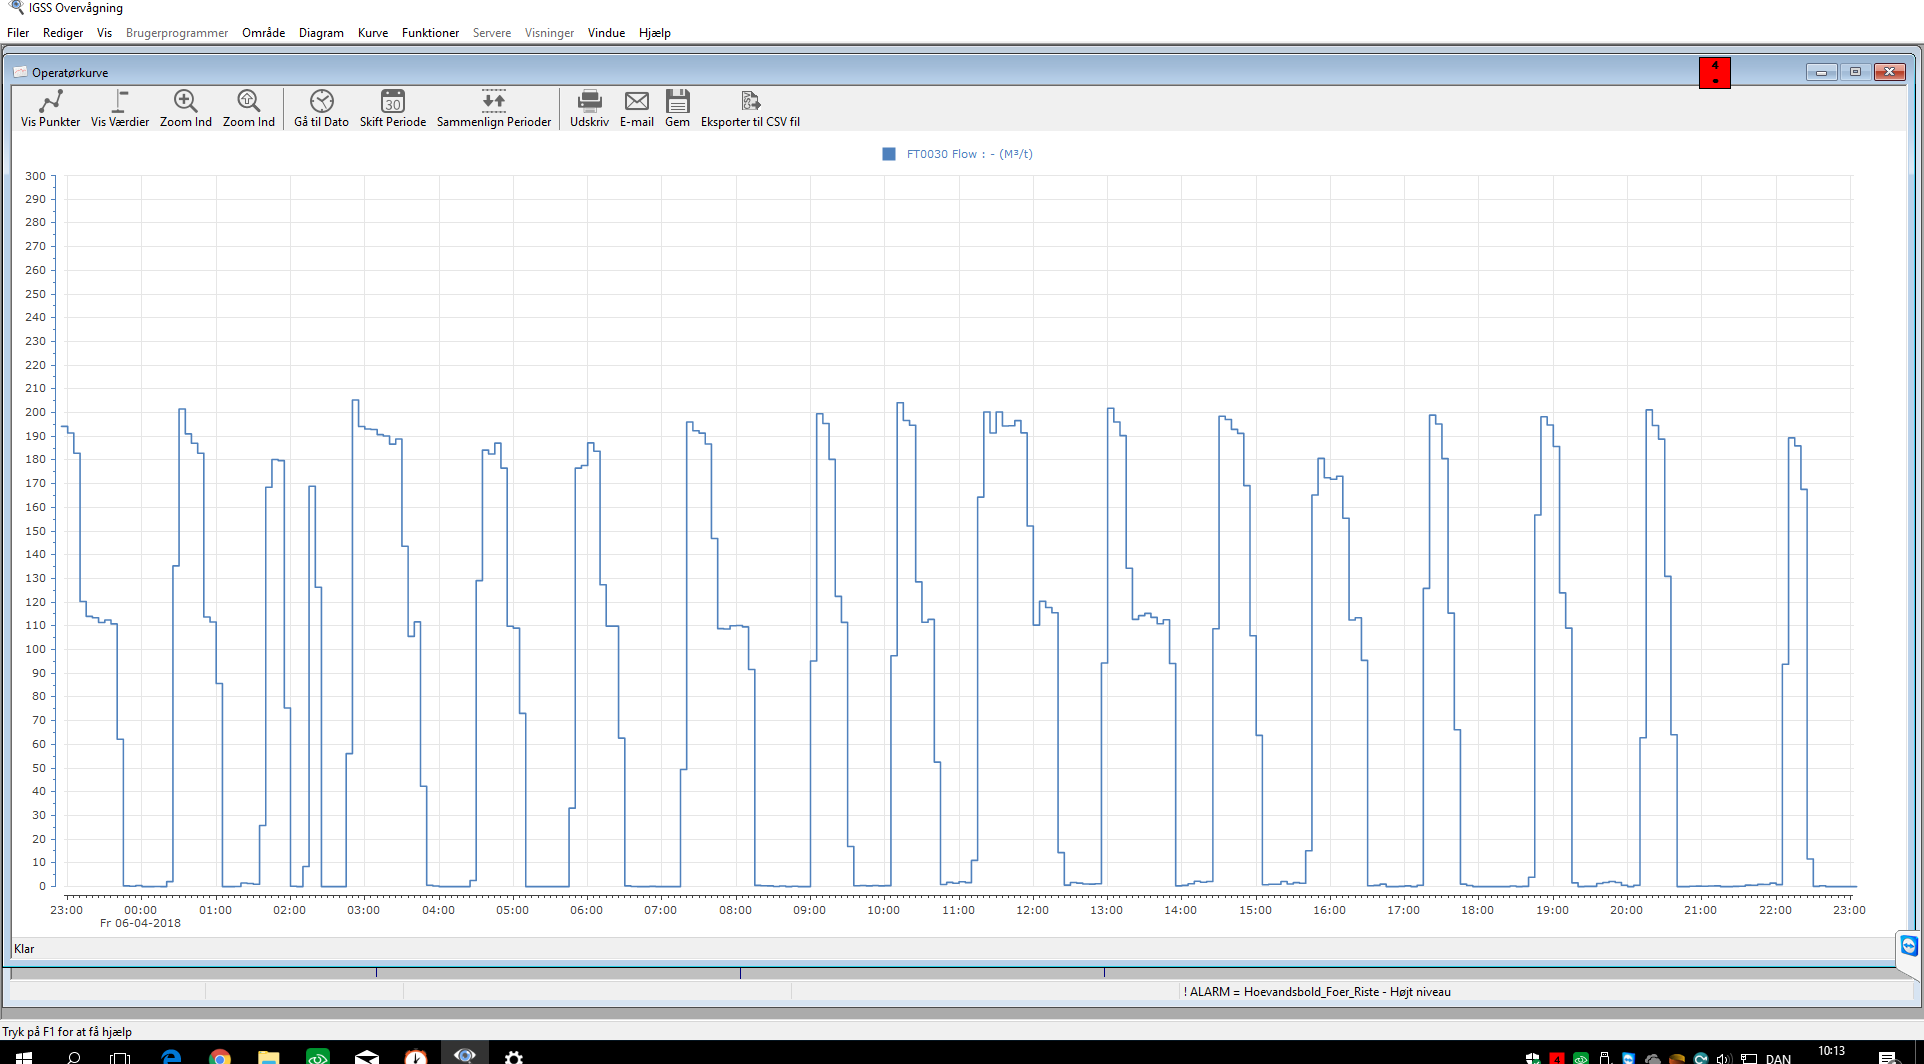
\includegraphics[width=0.7\textwidth]{Sections/pictures/Carlsberg_data.png}
		\end{figure}
		\begin{figure}[H]
			\centering
			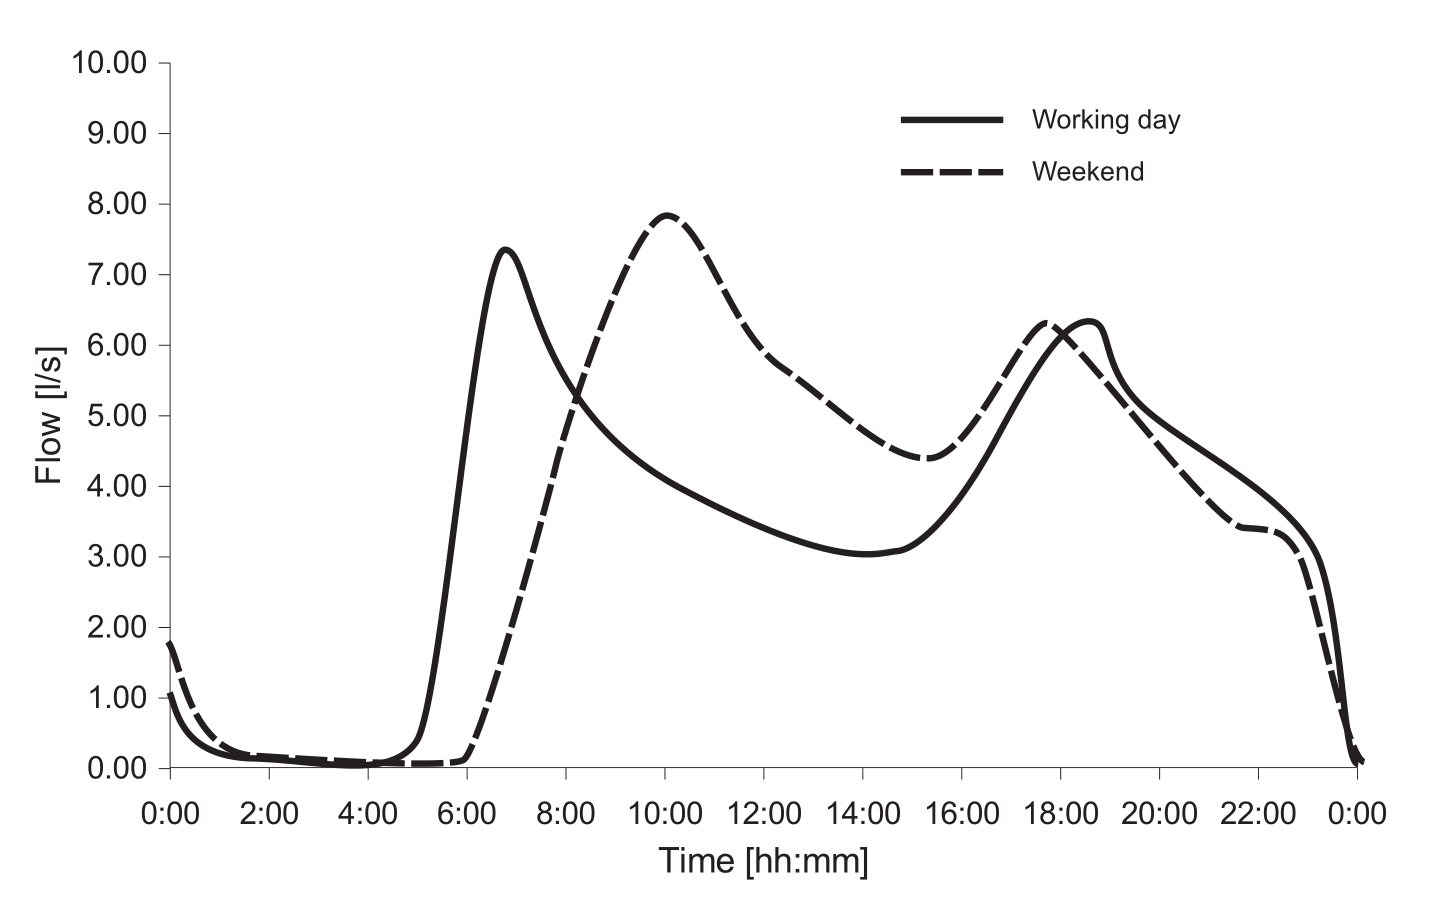
\includegraphics[width=0.7\textwidth]{Sections/pictures/poopflow.png}
		\end{figure}
	\end{column}
\end{columns}



\vfill\vfill	
\end{frame}

\subsection{Løsninger og begrænsninger}
\begin{frame}{Valg}{}
\vfill\vfill\centering
\begin{itemize}
	\item<1-> Indsættelse af tank.
	\item<2-> Afgrænse simulering til enkelt kemisk component.
	\item<3-> Runde kloak rør.
\end{itemize}
\vfill\vfill	
\end{frame}

\section{Modellering}

\begin{frame}{4 modeller}{}
	\vfill\vfill\centering
\begin{itemize}
	\item Kloak ledning.
	\item Transport af concentrat i kloak ledning.
	\item Sammenkobling af kloakledninger.
	\item Tank. 
\end{itemize}
\vfill\vfill		
\end{frame}

\begin{frame}{Kloak ledning}{Saint-Venant ligningerne}{}
	\vfill\vfill\centering
	
\begin{columns}
		\begin{column}{0.4\textwidth}
			\begin{itemize}
				\item<1-> $\dfrac{\partial A(x,t)}{\partial t} + \dfrac{\partial Q(x,t)}{\partial x}=0$
				\vspace{9mm}
				\item<2-> $\dfrac{1}{gA} \dfrac{\partial Q}{\partial t} +\dfrac{1}{gA}\dfrac{\partial}{\partial x} \left( \dfrac{Q^2}{A} \right) +
				\dfrac{\partial h}{\partial x} + S_f - S_b = 0$
				
				\vspace{9mm}
				\item<3-> Approksimationer af momentum ligningen.
				%\item<4-> Kinematisk bølge approksimation
			\end{itemize}
		\end{column}
		\begin{column}{0.48\textwidth}
			\begin{figure}[H]
				\centering
				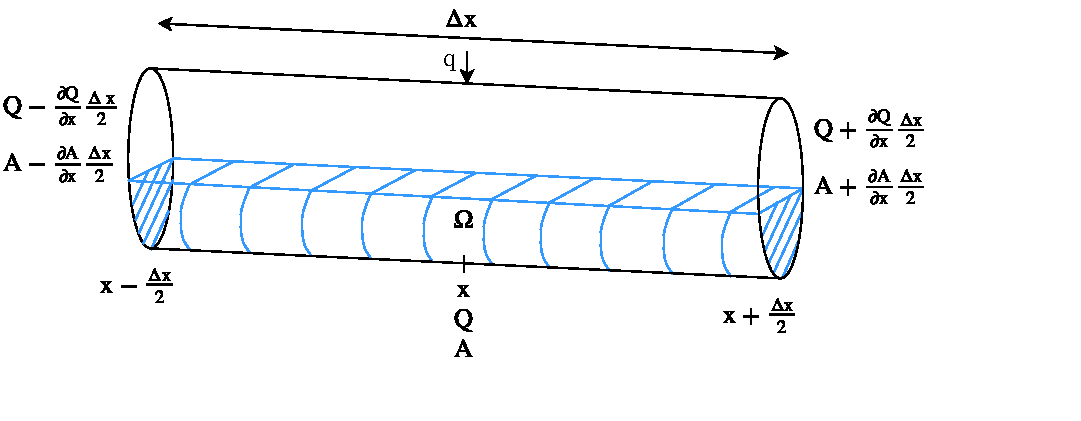
\includegraphics[width=1.2\textwidth]{Sections/pictures/continuity_open_channel.pdf}
			\end{figure}
		\end{column}
	\end{columns}
\vfill\vfill		
\end{frame}

\begin{frame}{Transport af koncentrat}{}
	\vfill\vfill\centering
\begin{columns}
	\begin{column}{0.4\textwidth}
		\begin{itemize}
			\vspace{9mm}
			\item<1-> $	A \cdot \dfrac{\partial C}{\partial t} + Q \cdot \dfrac{\partial C}{\partial x} = 0$
			\vspace{9mm}
			\item<2-> Afhænger af kendt $A$ og $Q$.
		\end{itemize}
	\end{column}
	
	\begin{column}{0.48\textwidth}
		\begin{figure}[H]
			\centering
			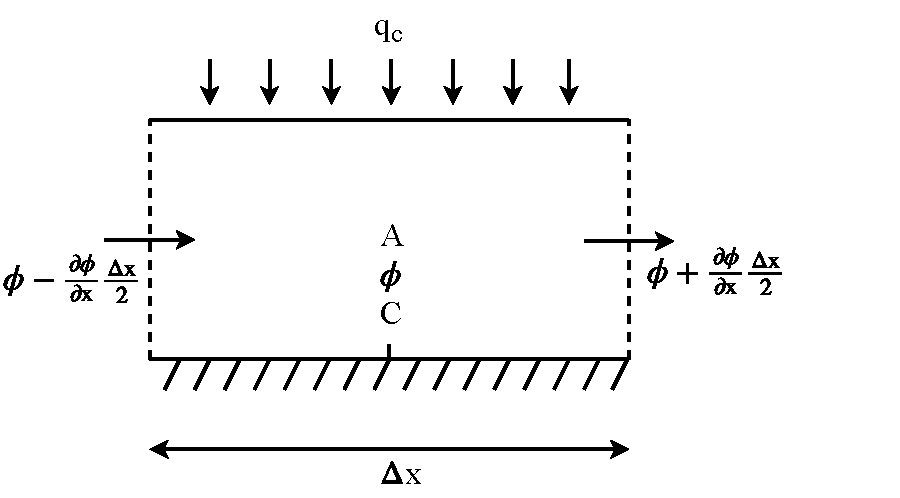
\includegraphics[width=1.1\textwidth]{Sections/pictures/poopvolume.pdf}
		\end{figure}
	\end{column}
\end{columns}


\vfill\vfill		
\end{frame}

\begin{frame}{Sammenkobling af kloak ledninger}{}
\vfill\vfill\centering
	\begin{columns}
	\begin{column}{0.4\textwidth}
		\begin{itemize}
			\vspace{9mm}
			\item<1-> $Q_3 = Q_1 + Q_2$
			\vspace{9mm}
			\item<2-> $C_3 = \dfrac{C_1 \cdot Q_1 + C_2 \cdot Q_2}{Q_1 + Q_2}$
		\end{itemize}
	\end{column}

	\begin{column}{0.48\textwidth}
		\begin{figure}[H]
			\centering
			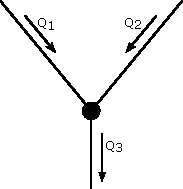
\includegraphics[width=0.7\textwidth]{Sections/pictures/interconnections.pdf}
		\end{figure}
	\end{column}
\end{columns}
\vfill\vfill		
\end{frame}

\begin{frame}{Tank}{}
\vfill\vfill\centering
	\begin{columns}
	\begin{column}{0.75\textwidth}
		\begin{itemize}
			\vspace{9mm}
			\item<1-> $\dfrac{dh(t)}{dt}=\dfrac{1}{A} \left(Q_{in}(t)-u(t) \cdot \overline Q \right)$
			\vspace{9mm}
			\item<2-> $\dfrac{dC_{tank}(t)}{dt} = \dfrac{1}{A} \left(C_{in}(t) \cdot \dfrac{Q_{in}(t)}{h(t)} - C_{tank}(t) \cdot \dfrac{Q_{out}(t)}{h(t)} \right)$
		\end{itemize}
	\end{column}

	\begin{column}{0.3\textwidth}
		\begin{figure}[H]
			\centering
			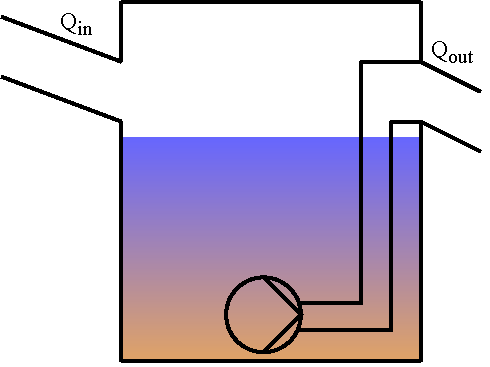
\includegraphics[width=0.9\textwidth]{Sections/pictures/reservior_with_pump.pdf}
		\end{figure}
	\end{column}
\end{columns}
\vfill\vfill		
\end{frame}
	
\section{Simulering}
\subsection{Struktur}
\begin{frame}{Tre dele}{}
\vfill\vfill\centering

\begin{itemize}
	\item \textbf{Intialisering}
	\item<1-> Opsætning af komponenter.
	\item<2-> System i steady state.
	\item<3-> \textbf{Simulering}
	\item<4-> Iterativ beregning af komponenterne
	\item<5-> \textbf{Gennemgang af resultat}
\end{itemize}

\vfill\vfill		
\end{frame}

\begin{frame}{Playback funktion}{}
\vfill\vfill\centering
		\begin{figure}[H]
			\centering
			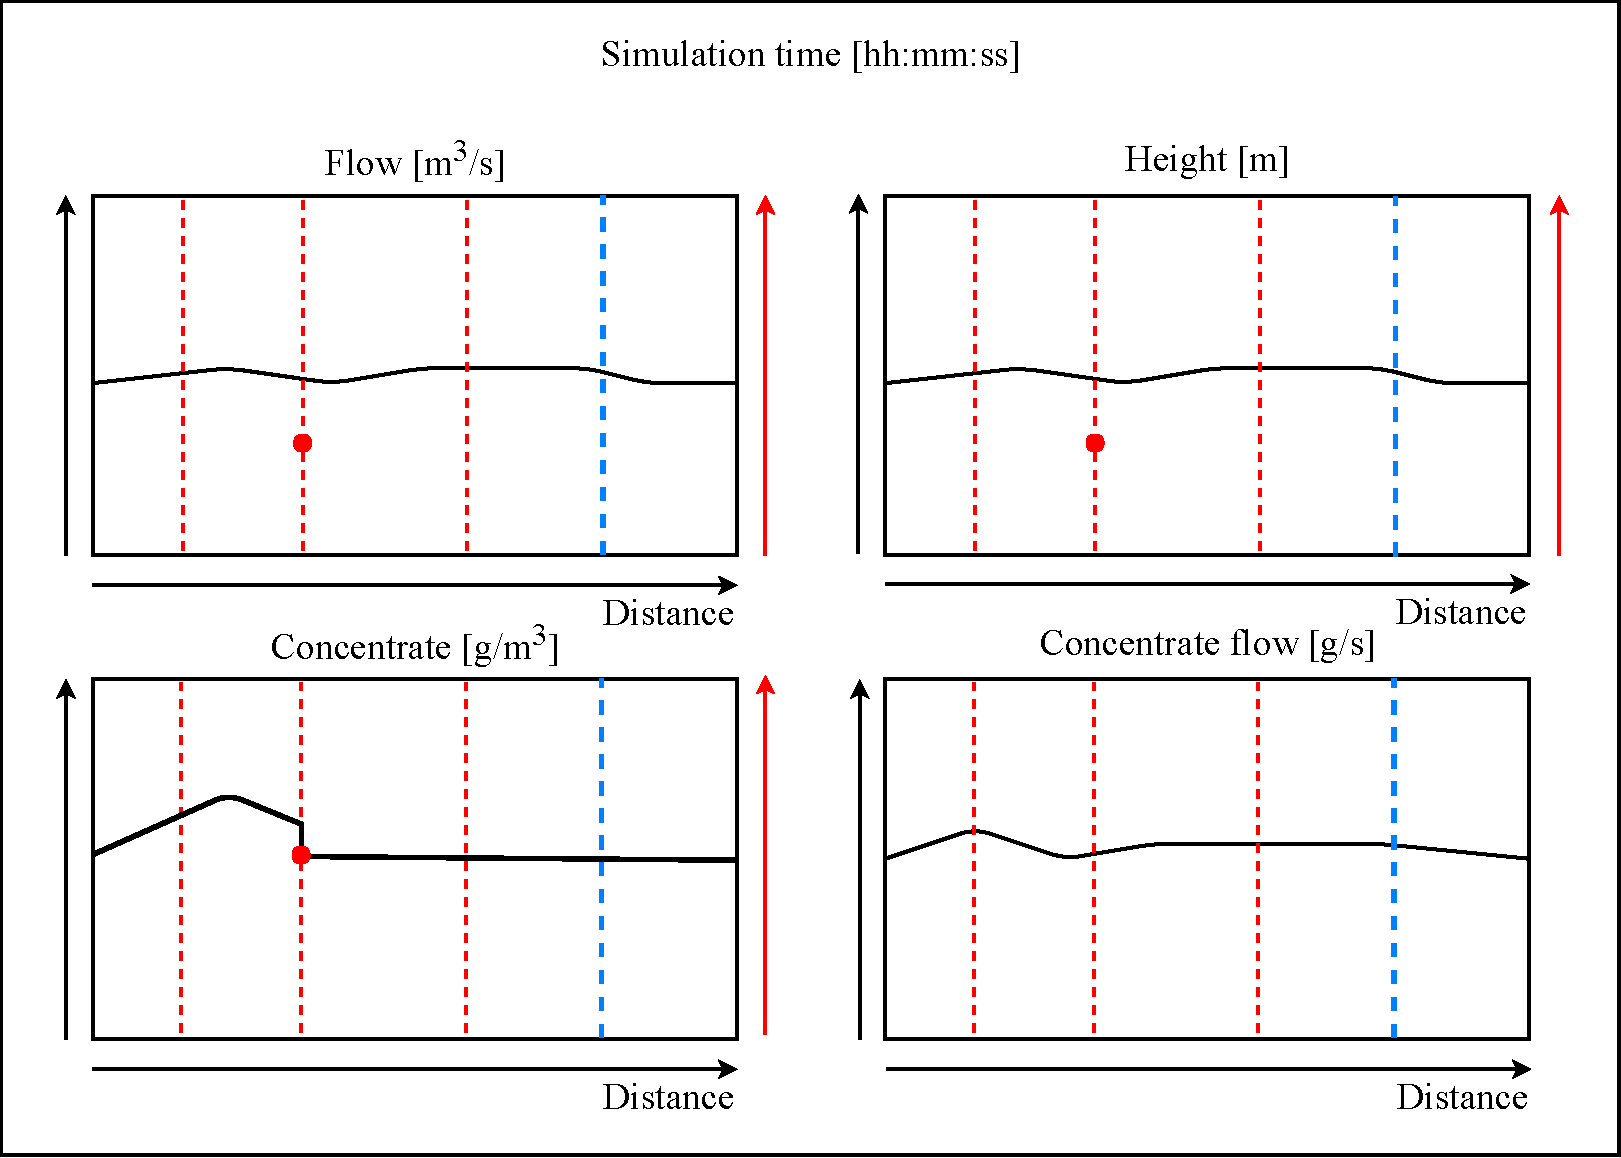
\includegraphics[width=0.7\textwidth]{Sections/pictures/display_results.pdf}
		\end{figure}
\vfill\vfill		
\end{frame}

\subsection{Preissmann}

\begin{frame}{Preissmann}{}
\vfill\vfill\centering
\begin{itemize}
	\item Kinematisk bølge aproksimering.
	\item Fyldningsgrad kurve for rør.
\end{itemize}
\vfill\vfill		
\end{frame}

\begin{frame}{Preissmann}{}
\vfill\vfill\centering
		\begin{figure}[H]
			\centering
			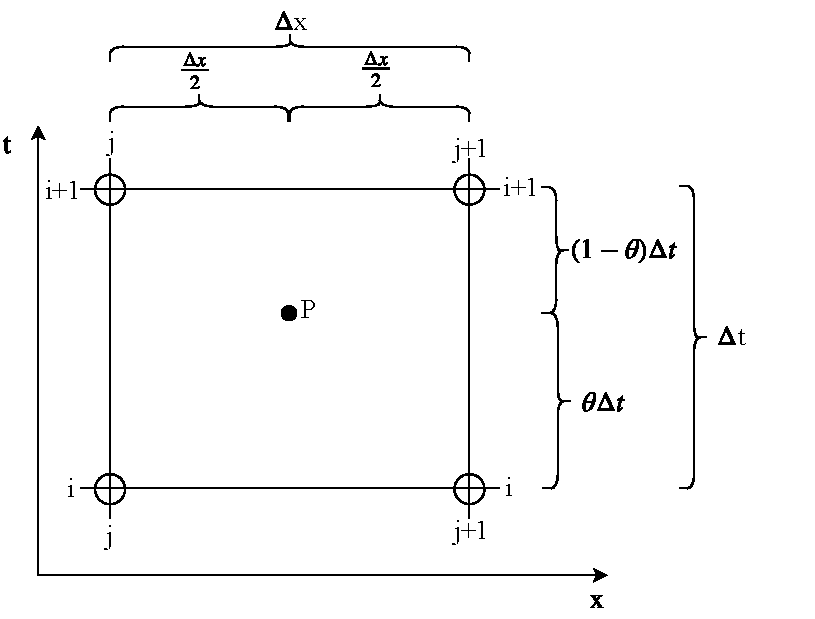
\includegraphics[width=0.7\textwidth]{Sections/pictures/preissmann_scheme.pdf}
		\end{figure}
\vfill\vfill		
\end{frame}

\begin{frame}{Preissmann iteration}{}
\vfill\vfill\centering
		\begin{figure}[H]
			\centering
			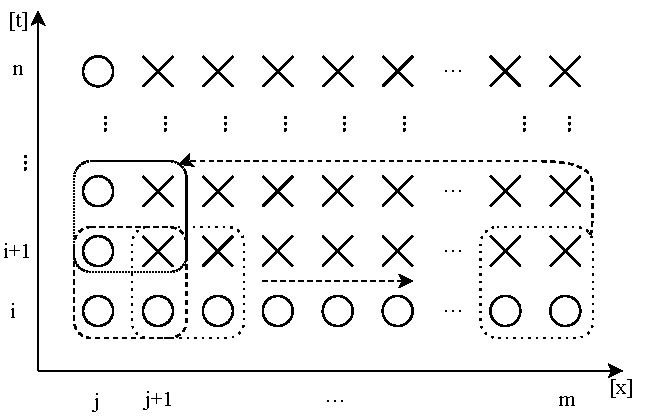
\includegraphics[width=0.7\textwidth]{Sections/pictures/preissmann_scheme_iteration.pdf}
		\end{figure}
\vfill\vfill		
\end{frame}

\begin{frame}{Preissmann stabilitet}{}
\vfill\vfill\centering
	\begin{columns}
		\begin{column}{0.25\textwidth}
		\vspace{20mm}
			\begin{itemize}
				\item Ubetinget stabilitet
			\end{itemize}
		\end{column}

		\begin{column}{0.7\textwidth}
			\begin{figure}[H]
	  			% This file was created by matlab2tikz.
%
%The latest updates can be retrieved from
%  http://www.mathworks.com/matlabcentral/fileexchange/22022-matlab2tikz-matlab2tikz
%where you can also make suggestions and rate matlab2tikz.
%
\definecolor{mycolor1}{rgb}{0.00000,0.44700,0.74100}%
\definecolor{mycolor2}{rgb}{0.85000,0.32500,0.09800}%
\definecolor{mycolor3}{rgb}{0.92900,0.69400,0.12500}%
%

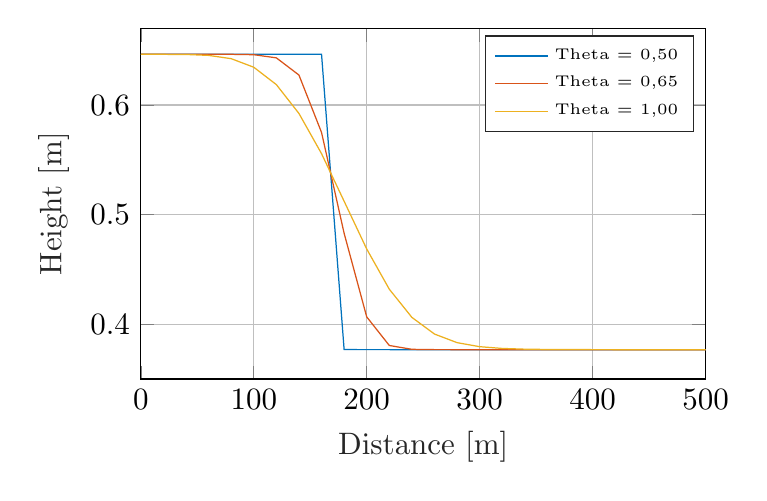
\begin{tikzpicture}[scale=1.12]

\begin{axis}[%
width=2.521in,
height=1.566in,
at={(0.758in,0.481in)},
scale only axis,
xmin=0,
xmax=500,
xlabel style={font=\color{white!15!black}},
xlabel={Distance [m]},
ymin=0.35,
ymax=0.67,
ylabel style={font=\color{white!15!black}},
ylabel={Height [m]},
axis background/.style={fill=white},
xmajorgrids,
ymajorgrids,
legend style={legend cell align=left, align=left, font=\tiny, draw=white!15!black}
]
\addplot [color=mycolor1]
  table[row sep=crcr]{%
0	0.646320000000003\\
60	0.646276050713254\\
160	0.646310155623098\\
180	0.376872286030618\\
280	0.376840431718108\\
500	0.376840417593883\\
};
\addlegendentry{Theta = 0,50}

\addplot [color=mycolor2]
  table[row sep=crcr]{%
0	0.646320000000003\\
80	0.64624640057724\\
100	0.645897528752698\\
120	0.643024844027934\\
140	0.627340662030861\\
160	0.574962749099655\\
180	0.482975200012561\\
200	0.406738255140283\\
220	0.380633403616173\\
240	0.377144178424658\\
260	0.376861538074763\\
400	0.376840417642768\\
500	0.376840417593883\\
};
\addlegendentry{Theta = 0,65}

\addplot [color=mycolor3]
  table[row sep=crcr]{%
0	0.646320000000003\\
40	0.646114001556498\\
60	0.645277732382112\\
80	0.642278908735364\\
100	0.634470248439527\\
120	0.618608579564977\\
140	0.592296821259026\\
160	0.555638802949943\\
180	0.512224654573913\\
200	0.468642227745363\\
220	0.431975238240568\\
240	0.406279099337155\\
260	0.391077260818861\\
280	0.383229133040004\\
300	0.379555033462054\\
320	0.377947501212986\\
340	0.377277301724973\\
360	0.377008073659567\\
400	0.376863443115042\\
500	0.376840600709272\\
};
\addlegendentry{Theta = 1,00}

\end{axis}
\end{tikzpicture}%
			\end{figure}
		\end{column}
	\end{columns}			
\vfill\vfill		
\end{frame}



\begin{frame}{Courant's tal}{}
\vfill\vfill\centering

\begin{itemize}
	\item<1-> Indikation af præcision  
	\item<2-> $C_r =  \dfrac{\sqrt{g \cdot \overline{\text{H}}} \cdot \Delta t}{\Delta x}$ 
\end{itemize}

\vfill\vfill		
\end{frame}

\begin{frame}{Courant's tal}{}
\vfill\vfill\centering
\begin{figure}[H]
  % This file was created by matlab2tikz.
%
%The latest updates can be retrieved from
%  http://www.mathworks.com/matlabcentral/fileexchange/22022-matlab2tikz-matlab2tikz
%where you can also make suggestions and rate matlab2tikz.
%
\definecolor{mycolor1}{rgb}{0.00000,0.44700,0.74100}%
\definecolor{mycolor2}{rgb}{0.85000,0.32500,0.09800}%
\definecolor{mycolor3}{rgb}{0.92900,0.69400,0.12500}%
\definecolor{mycolor4}{rgb}{0.49400,0.18400,0.55600}%
\definecolor{mycolor5}{rgb}{0.46600,0.67400,0.18800}%
%
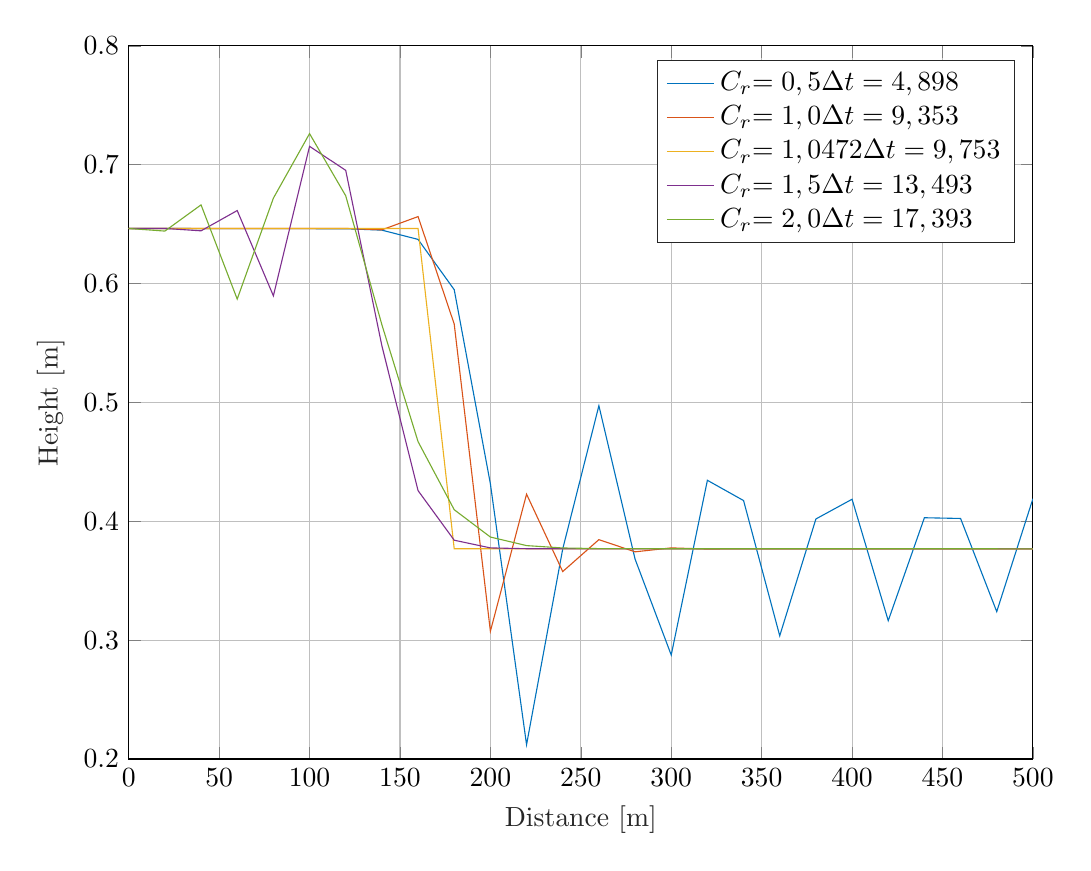
\begin{tikzpicture}

\begin{axis}[%
width=4.521in,
height=3.566in,
at={(0.758in,0.481in)},
scale only axis,
xmin=0,
xmax=500,
xlabel style={font=\color{white!15!black}},
xlabel={Distance [m]},
ymin=0.2,
ymax=0.8,
ylabel style={font=\color{white!15!black}},
ylabel={Height [m]},
axis background/.style={fill=white},
xmajorgrids,
ymajorgrids,
legend style={legend cell align=left, align=left, draw=white!15!black}
]
\addplot [color=mycolor1]
  table[row sep=crcr]{%
0	0.646320000000003\\
120	0.646110798810184\\
140	0.644921440462895\\
160	0.637135852956419\\
180	0.594824492956263\\
200	0.43150901335224\\
220	0.212065679465525\\
240	0.376715133178777\\
260	0.497228602202995\\
280	0.368225074016379\\
300	0.287474004612932\\
320	0.434471939483103\\
340	0.417428829121661\\
360	0.303655446833545\\
380	0.401943487002541\\
400	0.418541170475294\\
420	0.31638041784953\\
440	0.402974501738697\\
460	0.402359479024142\\
480	0.323982099181592\\
500	0.418993270269539\\
};
\addlegendentry{$\text{C}_\text{r}\text{ = 0,5 }\Delta\text{t = 4,898}$}

\addplot [color=mycolor2]
  table[row sep=crcr]{%
0	0.646320000000003\\
100	0.64627269447675\\
120	0.646347802512935\\
140	0.645200955430653\\
160	0.656315606992678\\
180	0.565887713400684\\
200	0.307486457782431\\
220	0.422792612949024\\
240	0.357707826201363\\
260	0.384552559769702\\
280	0.374292850753534\\
300	0.377612917409238\\
320	0.376627578465389\\
340	0.376895037076054\\
420	0.376840400054334\\
500	0.376840417594508\\
};
\addlegendentry{$\text{C}_\text{r}\text{ = 1,0 }\Delta\text{t = 9,353}$}

\addplot [color=mycolor3]
  table[row sep=crcr]{%
0	0.646320000000003\\
120	0.646276927816245\\
160	0.646310155623098\\
180	0.376872286030618\\
360	0.376840417591211\\
500	0.376840417593883\\
};
\addlegendentry{$\text{C}_\text{r}\text{ = 1,0472 }\Delta\text{t = 9,753}$}

\addplot [color=mycolor4]
  table[row sep=crcr]{%
0	0.646320000000003\\
20	0.646369888199388\\
40	0.644339908290192\\
60	0.661409073127913\\
80	0.589657421125025\\
100	0.715402174481824\\
120	0.695236626193719\\
140	0.547617729801175\\
160	0.42579367994415\\
180	0.384067663660119\\
200	0.377602369794033\\
220	0.376914145050648\\
300	0.376840453623174\\
500	0.376840417544031\\
};
\addlegendentry{$\text{C}_\text{r}\text{ = 1,5 }\Delta\text{t = 13,493}$}

\addplot [color=mycolor5]
  table[row sep=crcr]{%
0	0.646320000000003\\
20	0.644131656564412\\
40	0.666181907491705\\
60	0.586925572641576\\
80	0.671829743861394\\
100	0.726113397608458\\
120	0.673833056042724\\
140	0.565341030706179\\
160	0.466990002688476\\
180	0.409725577192091\\
200	0.386732102666656\\
220	0.379534757839167\\
240	0.377540174675403\\
260	0.377017102005198\\
320	0.376843047670491\\
500	0.376840416619302\\
};
\addlegendentry{$\text{C}_\text{r}\text{ = 2,0 }\Delta\text{t = 17,393}$}

\end{axis}
\end{tikzpicture}%
\end{figure}
\vfill\vfill		
\end{frame}

\begin{frame}{Courant's tal}{}
\vfill\vfill\centering
\begin{figure}[H]
  % This file was created by matlab2tikz.
%
%The latest updates can be retrieved from
%  http://www.mathworks.com/matlabcentral/fileexchange/22022-matlab2tikz-matlab2tikz
%where you can also make suggestions and rate matlab2tikz.
%
\definecolor{mycolor1}{rgb}{0.00000,0.44700,0.74100}%
\definecolor{mycolor2}{rgb}{0.85000,0.32500,0.09800}%
\definecolor{mycolor3}{rgb}{0.92900,0.69400,0.12500}%
\definecolor{mycolor4}{rgb}{0.49400,0.18400,0.55600}%
\definecolor{mycolor5}{rgb}{0.46600,0.67400,0.18800}%
%

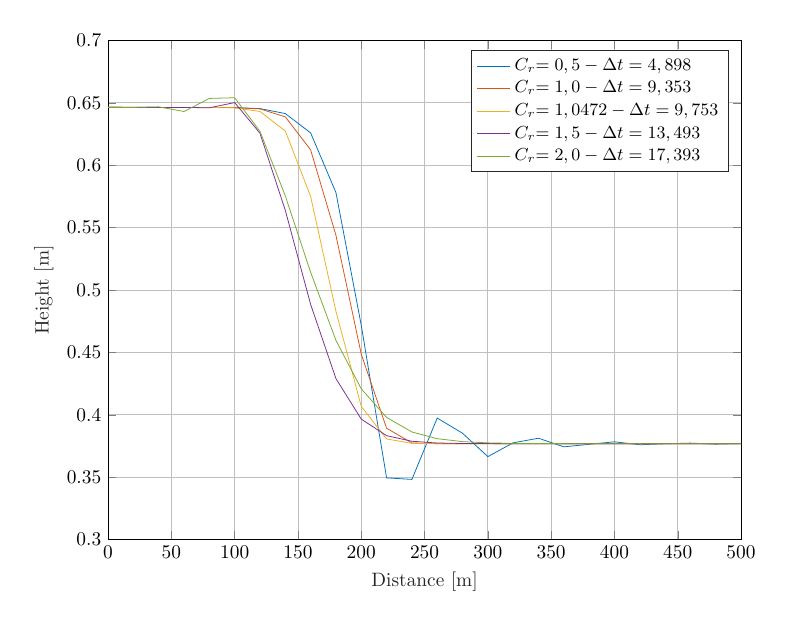
\begin{tikzpicture}[scale=0.7]

\begin{axis}[%
width=4.521in,
height=3.566in,
at={(0.758in,0.481in)},
scale only axis,
xmin=0,
xmax=500,
xlabel style={font=\color{white!15!black}},
xlabel={Distance [m]},
ymin=0.3,
ymax=0.7,
ylabel style={font=\color{white!15!black}},
ylabel={Height [m]},
axis background/.style={fill=white},
xmajorgrids,
ymajorgrids,
legend style={legend cell align=left, align=left, font=\small, draw=white!15!black}
]
\addplot [color=mycolor1]
  table[row sep=crcr]{%
0	0.646320000000003\\
100	0.646130379406088\\
120	0.645319736563408\\
140	0.641349626186809\\
160	0.625859263920574\\
180	0.578058697332551\\
200	0.471670741775881\\
220	0.349470522572005\\
240	0.348227708429135\\
260	0.397395101255427\\
280	0.385197584532591\\
300	0.36649580140255\\
320	0.377549288468572\\
340	0.381224116036606\\
360	0.374323450759618\\
400	0.378357325031061\\
420	0.375997243453128\\
440	0.376767504712859\\
460	0.377314673015633\\
480	0.376460343366603\\
500	0.376957947916708\\
};
\addlegendentry{$\text{C}_\text{r}\text{ = 0,5 } - \Delta\text{t = 4,898}$}

\addplot [color=mycolor2]
  table[row sep=crcr]{%
0	0.646320000000003\\
100	0.646142506713147\\
120	0.645085940723106\\
140	0.638714914649881\\
160	0.612308851353646\\
180	0.543809382353174\\
200	0.448609289609578\\
220	0.389253299316294\\
240	0.377444595181146\\
260	0.376856539679238\\
460	0.376840417593883\\
500	0.376840417593883\\
};
\addlegendentry{$\text{C}_\text{r}\text{ = 1,0 } - \Delta\text{t = 9,353}$}

\addplot [color=mycolor3]
  table[row sep=crcr]{%
0	0.646320000000003\\
80	0.646246242896211\\
100	0.645897359270862\\
120	0.643024752804138\\
140	0.627340728165507\\
160	0.57496313805126\\
180	0.48297580798635\\
200	0.406738381000366\\
220	0.380633284310363\\
240	0.377144123492656\\
260	0.376861434510261\\
420	0.376840417594337\\
500	0.376840417593883\\
};
\addlegendentry{$\text{C}_\text{r}\text{ = 1,0472 } - \Delta\text{t = 9,753}$}

\addplot [color=mycolor4]
  table[row sep=crcr]{%
0	0.646320000000003\\
60	0.646287714980758\\
80	0.645974039633757\\
100	0.650154622142281\\
120	0.625589872774526\\
140	0.563793095912615\\
160	0.488461885784659\\
180	0.42899697304307\\
200	0.396520148575974\\
220	0.383281578277945\\
240	0.378786168330805\\
260	0.377400896181314\\
280	0.376996576980616\\
320	0.376851653469316\\
500	0.376840417670735\\
};

\addlegendentry{$\text{C}_\text{r}\text{ = 1,5 } - \Delta\text{t = 13,493}$}

\addplot [color=mycolor5]
  table[row sep=crcr]{%
0	0.646320000000003\\
20	0.646253446790183\\
40	0.646741328354437\\
60	0.642999942630581\\
80	0.653489860013963\\
100	0.65401950972398\\
120	0.62704350368125\\
140	0.575366566439072\\
160	0.514211327388352\\
180	0.459639658549975\\
200	0.420783611238903\\
220	0.397904618644986\\
240	0.386245066973913\\
260	0.380849107690779\\
280	0.378497038184321\\
300	0.377509898191704\\
320	0.377106256296543\\
360	0.376880597240245\\
500	0.376840457105232\\
};

\addlegendentry{$\text{C}_\text{r}\text{ = 2,0 } - \Delta\text{t = 17,393}$}

\end{axis}
\end{tikzpicture}%
\end{figure}
\vfill\vfill		
\end{frame}



